
\usetikzlibrary {positioning}
\newcommand{\ModelColor}{red}
\newcommand{\UserInterfaceColor}{yellow}
\newcommand{\PersistenceColor}{blue}
\newcommand{\PointerSwapColor}{green}
\newcommand{\OrchestratorColor}{blue}

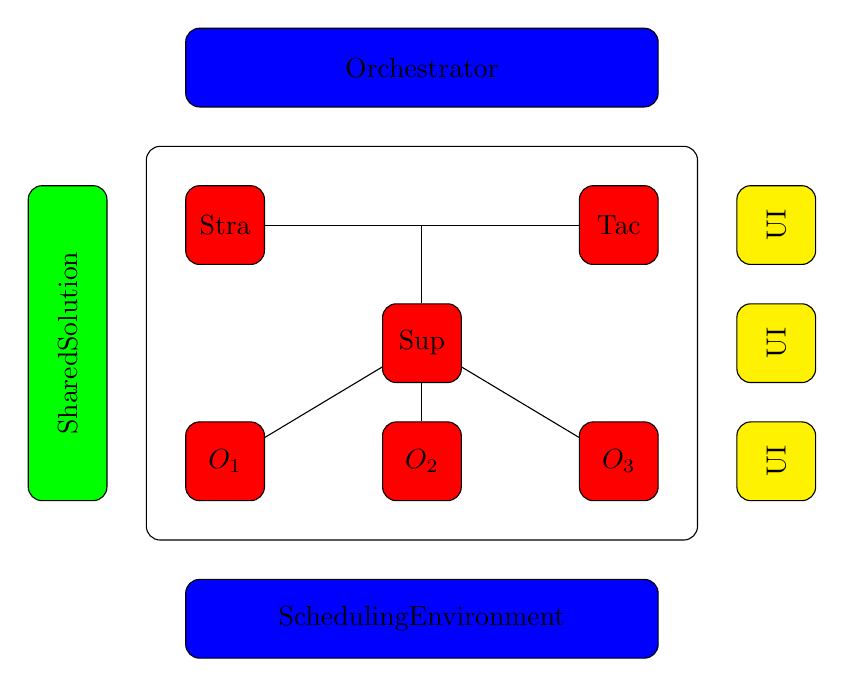
\begin{tikzpicture}[
	% Define styles and settings
	node distance=2cm,
	block/.style={rectangle, draw, fill=blue!20, text centered, minimum height=3em},
	arrow/.style={-Stealth, thick}
	]
	% \draw[help lines] (0, 0) grid (10, 8);
  
	\draw (5,4) node[minimum height=5cm,minimum width=7.0cm,draw,rounded corners=5pt] {};

	    \draw (2.5,5.5) node[minimum height=1cm,minimum width=1cm,draw,fill=\ModelColor,rounded corners=5pt] (Strategic) {Stra};
	    \draw (5.0,4.0) node[minimum height=1cm,minimum width=1cm,draw,fill=\ModelColor,rounded corners=5pt] (Supervisor) {Sup};
		\draw (7.5,5.5) node[minimum height=1cm,minimum width=1cm,draw,fill=\ModelColor,rounded corners=5pt] (Tactical) {Tac};

		\draw (2.5,2.5) node[minimum height=1cm,minimum width=1cm,draw,fill=\ModelColor,rounded corners=5pt] (Operational_1) {$O_{1}$};
		\draw (5.0,2.5) node[minimum height=1cm,minimum width=1cm,draw,fill=\ModelColor,rounded corners=5pt] (Operational_2) {$O_{2}$};
		\draw (7.5,2.5) node[minimum height=1cm,minimum width=1cm,draw,fill=\ModelColor,rounded corners=5pt,rounded corners=5pt] (Operational_3) {$O_{3}$};
		
		\draw (Strategic) edge (Tactical);

		\draw (Strategic) edge (Tactical);
		\draw (5,5.5) edge (Supervisor);

		\draw (Supervisor) edge (Operational_1);
		\draw (Supervisor) edge (Operational_2);
		\draw (Supervisor) edge (Operational_3);
	\draw (5,0.5) node[minimum height=1cm,minimum width=6cm,draw,fill=\PersistenceColor,rounded corners=5pt] {SchedulingEnvironment};
	\draw (5,7.5) node[minimum height=1cm,minimum width=6cm,draw,fill=\OrchestratorColor,rounded corners=5pt] {Orchestrator};
	\draw (0.5,4) node[rotate=90, minimum height=1cm, minimum width=4cm,draw,fill=\PointerSwapColor,rounded corners=5pt] {SharedSolution};
	\draw (9.5,5.5) node[rotate=90, minimum height=1cm, minimum width=1cm,draw,fill=\UserInterfaceColor,rounded corners=5pt] {UI};
	\draw (9.5,4) node[rotate=90, minimum height=1cm, minimum width=1cm,draw,fill=\UserInterfaceColor,rounded corners=5pt] {UI};
	\draw (9.5,2.5) node[rotate=90, minimum height=1cm, minimum width=1cm,draw,fill=\UserInterfaceColor,rounded corners=5pt] {UI};

\end{tikzpicture}
